\subsection{Simulation}

\subsubsection{Aufbau}

\newpage
\subsubsection{Reflexionskoeffizient}

\begin{figure}[h!]
	\centering
	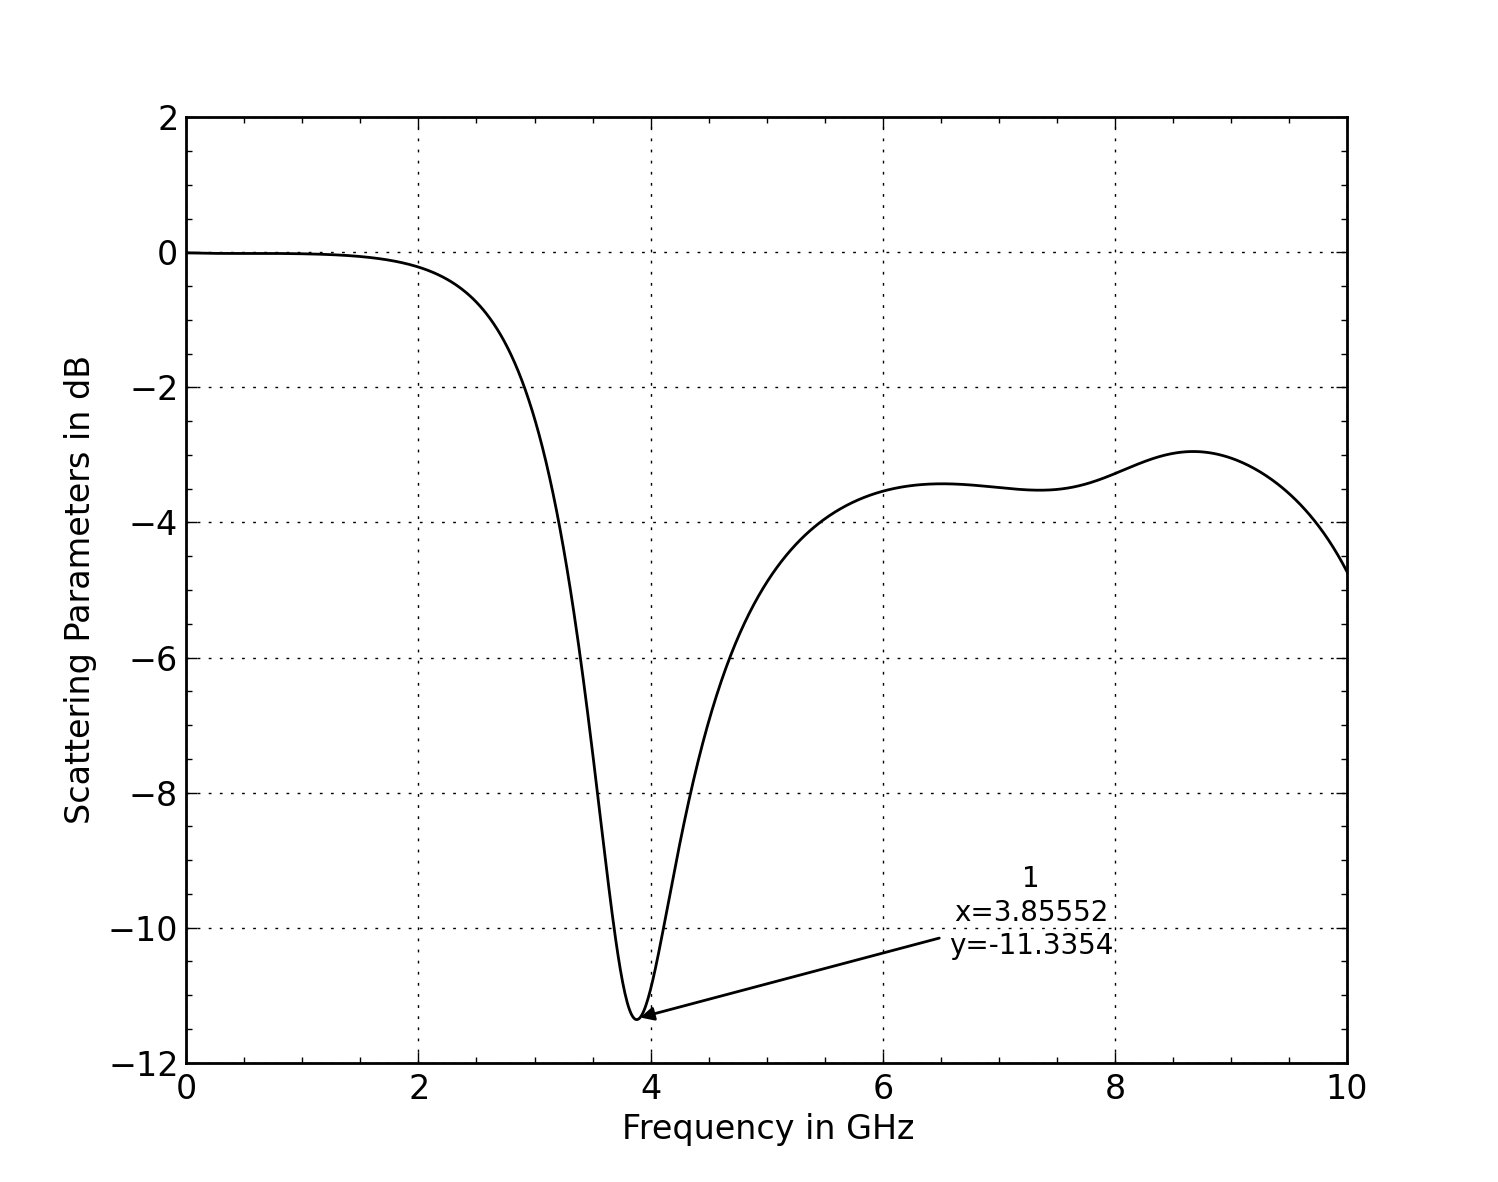
\includegraphics[width=0.75\textwidth]{../fig/plt/monopol_a_sim_s11.png}
	\caption{Reflexionskoeffizient ($S_{11}$ Parameter).}
\end{figure}

\newpage
\subsubsection{Antennenimpedanz}

\begin{figure}[h!]
	\centering
	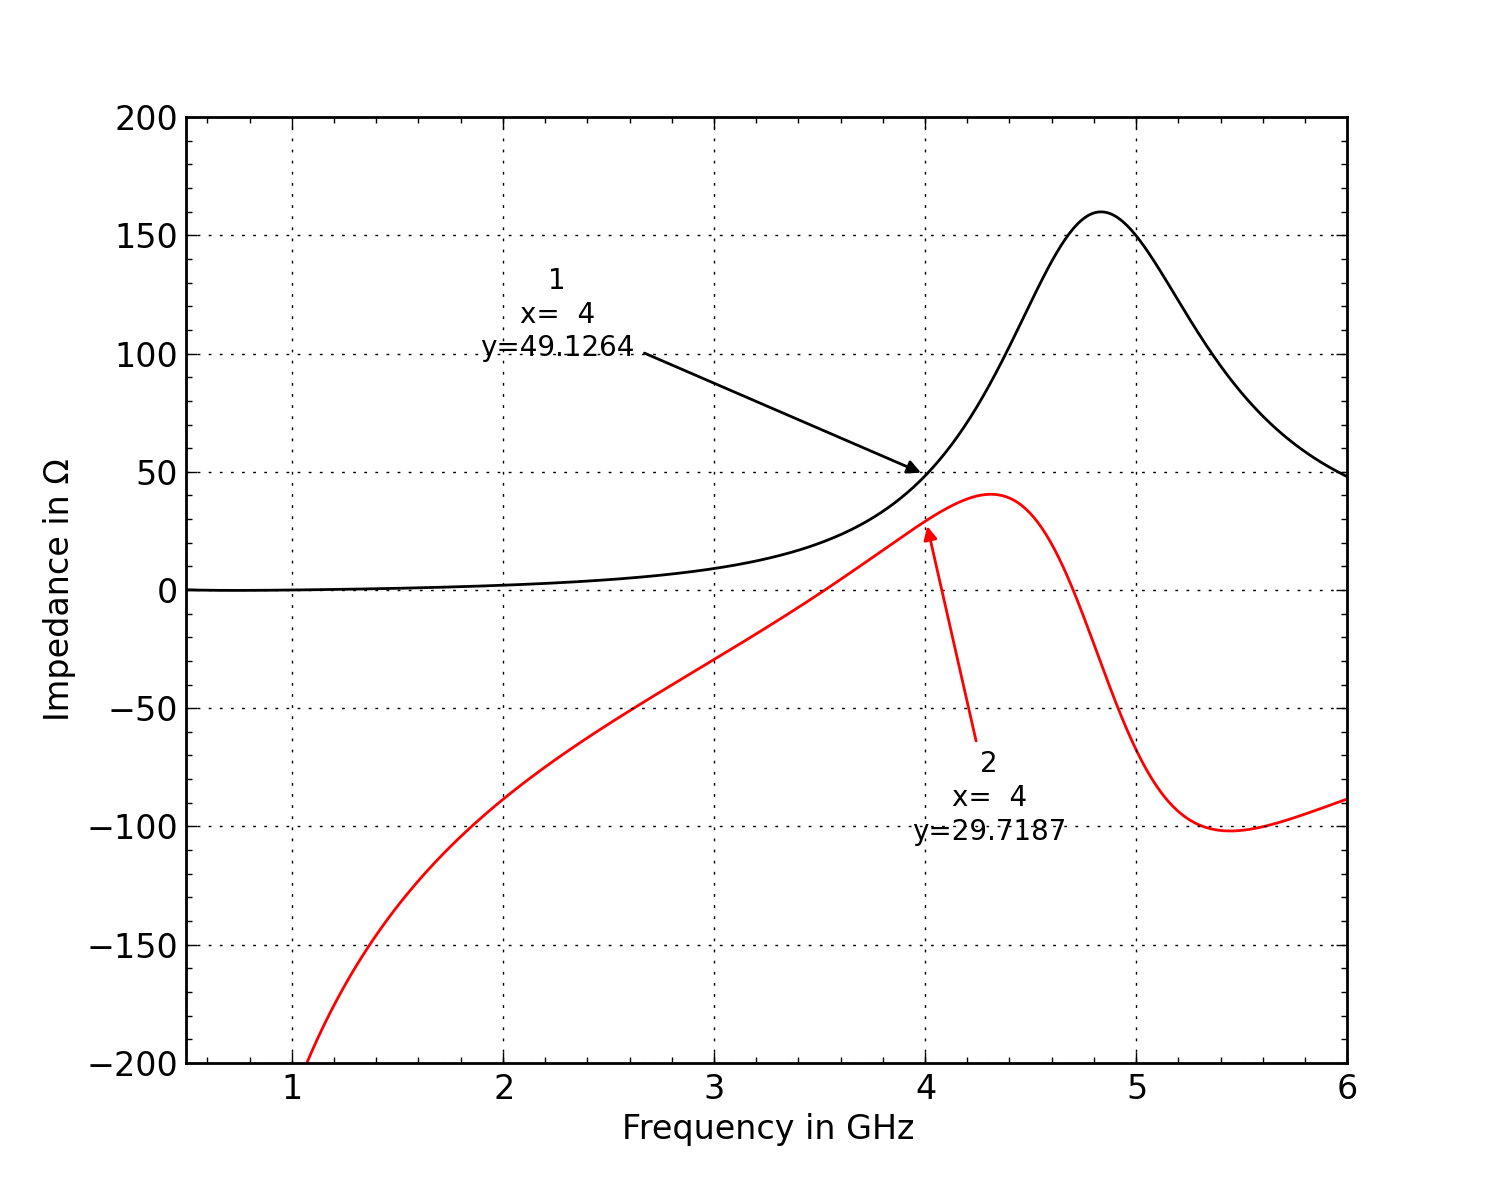
\includegraphics[width=0.75\textwidth]{../fig/plt/monopol_a_sim_impedance.png}
	\caption{Antennenimpedanz (Real- und Imaginäranteil).}
\end{figure}

\newpage
\subsubsection{2D Richtdiagramm}

\begin{figure}[h!]
	\centering
	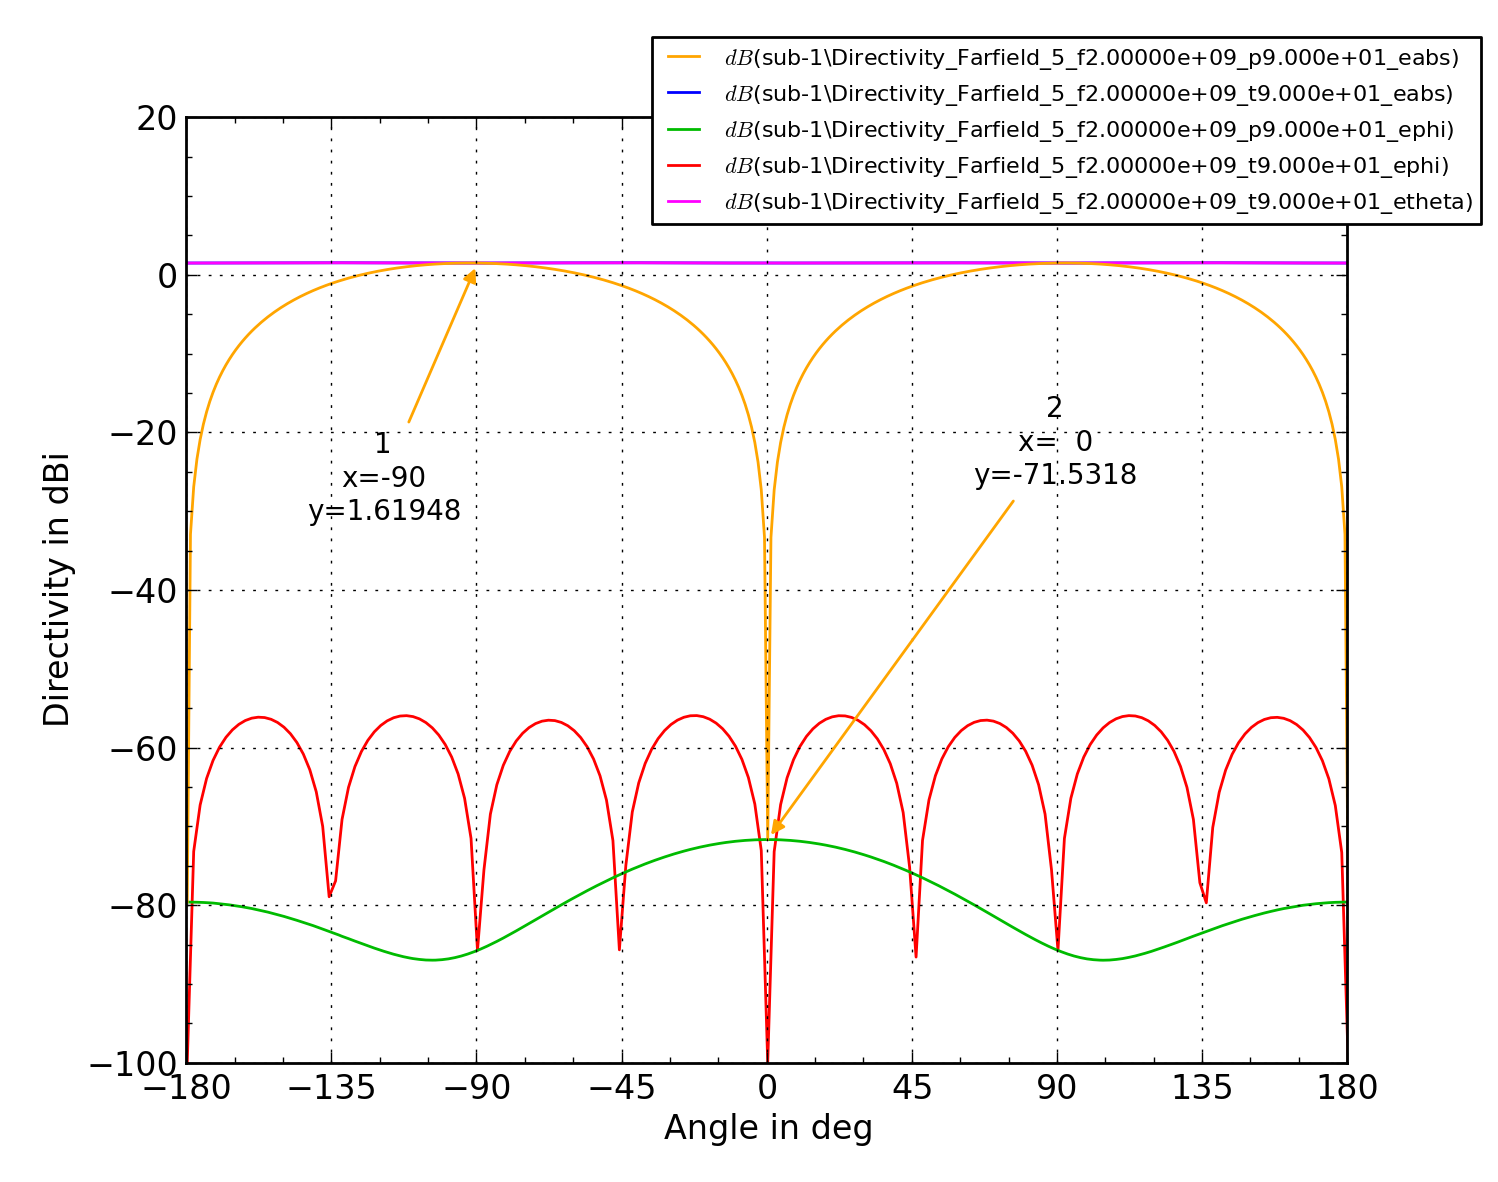
\includegraphics[width=0.75\textwidth]{../fig/plt/monopol_a_sim_2d_pattern.png}
	\caption{2D Richtdiagramm.}
\end{figure}

\newpage
\subsubsection{3D Richtdiagramm}

\begin{figure}[h!]
	\centering
	\begin{subfigure}[b]{0.48\textwidth}
		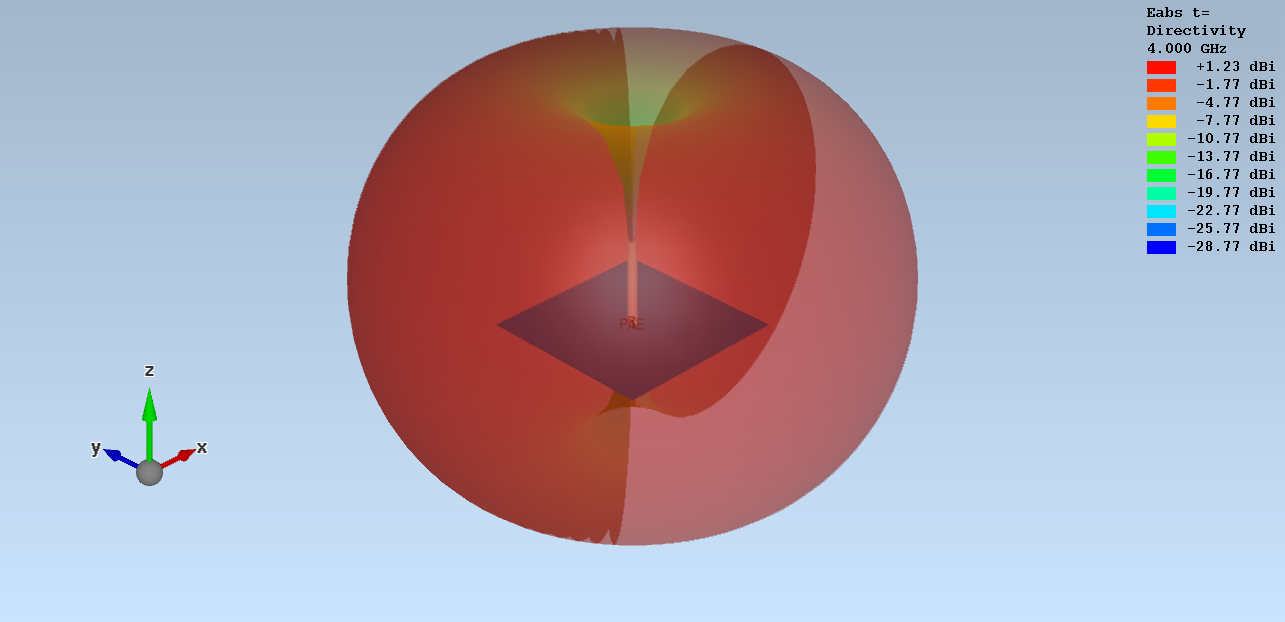
\includegraphics[width=1\textwidth]{../fig/plt/monopol_a_sim_3d_eabs.png}
		\caption{E-Feld Absolut}
	\end{subfigure}
	\begin{subfigure}[b]{0.48\textwidth}
		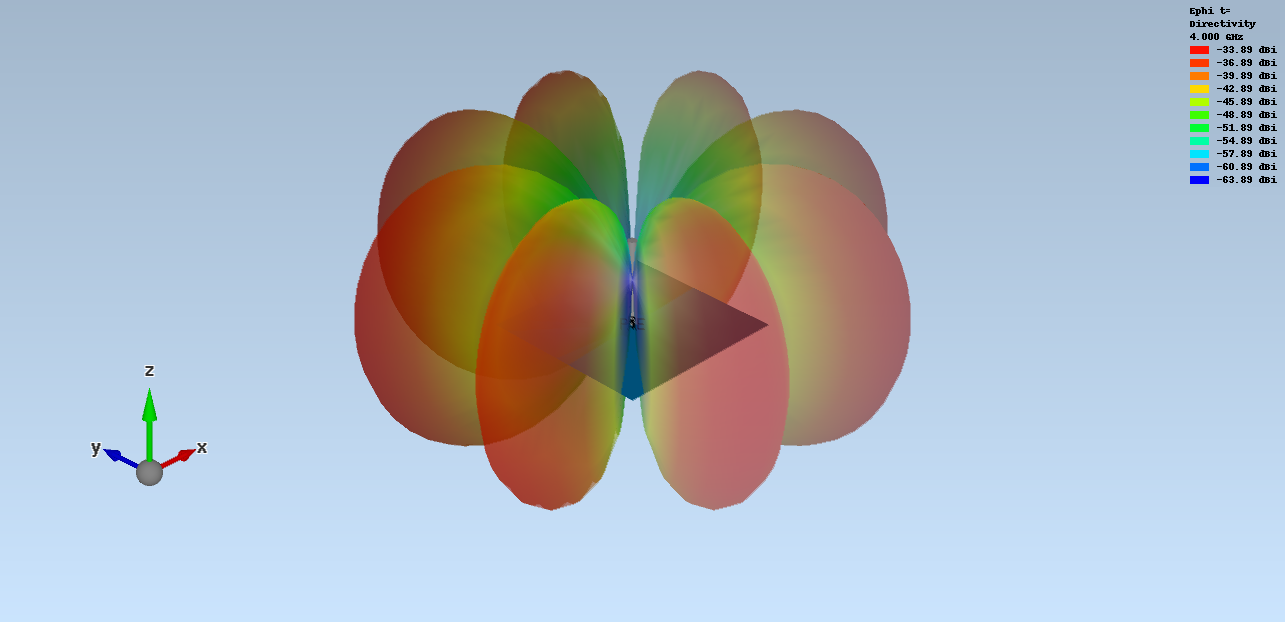
\includegraphics[width=1\textwidth]{../fig/plt/monopol_a_sim_3d_ephi.png}
		\caption{E-Feld $\varphi$}
	\end{subfigure}
	\caption{3D Darstellung des Fernfeldes}
	\label{fig:}
\end{figure}


